% FREUID Challenge 2026 - Technical Report (academic paper, built on the official template)
% Compile: pdflatex technical_report.tex && bibtex technical_report && pdflatex x2
%   (or:   latexmk -pdf technical_report.tex  /  tectonic -X compile technical_report.tex)
% Follows the organizers' one-column article template; figures are native TikZ/pgfplots.

\documentclass[11pt,a4paper]{article}

\usepackage[T1]{fontenc}
\usepackage[utf8]{inputenc}
\usepackage{lmodern}
\usepackage[htt]{hyphenat}   % allow \texttt tokens (pinned deps) to break at hyphens
\usepackage{microtype}
\usepackage{geometry}
\usepackage{graphicx}
\usepackage{booktabs}
\usepackage{float}
\usepackage{amsmath}
\usepackage{amssymb}
\usepackage{xcolor}
\usepackage{enumitem}
\usepackage{tikz}
\usetikzlibrary{arrows.meta,positioning,fit,backgrounds,calc}
\usepackage{pgfplots}
\pgfplotsset{compat=1.18}
\usepackage{caption}
\captionsetup{font=small,labelfont=bf}
\usepackage[hyphens]{url}
\usepackage{hyperref}
\usepackage{xurl}

\geometry{margin=2.5cm}
\hypersetup{
  colorlinks=true, breaklinks=true,
  linkcolor=blue!60!black, citecolor=blue!60!black, urlcolor=blue!60!black,
}
\emergencystretch=2.5em
\tolerance=1400
\hbadness=10000

% --- CVD-safe categorical palette (Okabe-Ito; validated dE 109.5, value labels give contrast relief) ---
\definecolor{cpub}{HTML}{0072B2}   % public-best model  (blue)
\definecolor{cpriv}{HTML}{E69F00}  % private-best model (orange)
\definecolor{axgray}{HTML}{6B6B6B}
\definecolor{gridgray}{HTML}{DCDCDC}
\definecolor{blockbg}{HTML}{EEF3F7}
\definecolor{tracebg}{HTML}{FBF0DF}

% --- recessive academic axis style ---
\pgfplotsset{
  paperaxis/.style={
    width=0.72\textwidth, height=5.2cm,
    axis line style={axgray, line width=0.5pt},
    tick style={axgray, line width=0.5pt},
    every tick label/.append style={font=\scriptsize, color=axgray},
    label style={font=\footnotesize},
    grid style={gridgray, line width=0.4pt},
    ymajorgrids=true, axis on top,
    legend style={font=\scriptsize, draw=axgray!60, fill=white, fill opacity=0.9,
                  text opacity=1, cells={anchor=west}},
  }
}

% --- template identity fields ---
\newcommand{\teamname}{ETRI\_MobilityAI}
\newcommand{\kaggleteam}{ETRI\_MobilityAI}
\newcommand{\contactemail}{syong.an@etri.re.kr}
\newcommand{\reportdate}{July 2026}

\title{%
  \textbf{Cross-Distribution Identity-Document Fraud Detection:\\
  Diversity-Axis Ensembles of Double-Trace Consistency Detectors}\\[0.5em]
  \large The FREUID Challenge 2026: Technical Report (Team \teamname)
}
\author{%
  Su-Yong An\thanks{Corresponding author: \texttt{syong.an@etri.re.kr}},
  \enspace Lae-Kyoung Lee\\
  \small
  Electronics and Telecommunications Research Institute (ETRI), Republic of Korea\\
  \texttt{\{syong.an,\,laeklee\}@etri.re.kr}
}
\date{Report date: \reportdate}

\begin{document}
\maketitle

\begin{abstract}
The FREUID Challenge 2026 requires a scalar fraud score in $[0,1]$ for each identity-document image, ranked
by the FREUID Score (AuDET $+$ APCER@1\%BPCER; lower is better). The test data has a deliberate distribution shift. The public split (about $5\%$ of the test data) is
born-digital. The private split (about $95\%$) decides the ranking. It is drawn from a hybrid of synthetic
and physically captured images, and it includes two document types absent from training. A single
submission is scored on both splits, and the private split dominates. The FREUID Score is a strict-tail
metric, so it punishes any subpopulation on which a model collapses. We therefore submit one model that is
built for robustness to captured and unseen-type content, not the model that tops the born-digital public
leaderboard. The submitted model is a Double-Trace Consistency (DTC) capture ensemble. Each DTC detector
adds a high-pass forensic branch to a pretrained RGB backbone and uses the trace twice: as a global feature
and as a document-type-agnostic patch-consistency signal. The main gain comes from ensembling backbones
that are decorrelated along two independent axes (architecture family and input resolution), not from extra
seeds; this reduces a two-backbone baseline from $0.354$ to about $0.22$--$0.27$ on a leakage-free captured
proxy. For comparison, a public-leaderboard-optimised ensemble reaches $0.00041$ on the public split but
collapses to near chance on captured data, which is why we do not submit it. All training uses competition
data and self-supervised augmentation only. Inference is a plain probability average with no test-time
parameter fitting, packaged in a pinned container that runs fully offline.
\end{abstract}

\noindent\textbf{Competition:} The FREUID Challenge 2026 (IJCAI-ECAI 2026), Kaggle
\texttt{the-freuid-challenge-2026-ijcai-ecai}~\cite{freuid2026}\\
\textbf{Kaggle team:} \kaggleteam\\
\textbf{Code:} \url{https://github.com/hoppery/freuid-challenge-2026}\\

\section{Introduction}
\label{sec:intro}
Identity-document fraud has several threat models: physical manipulation and re-capture, localized digital
editing, and fully synthetic (GenAI) content. The FREUID Challenge~\cite{freuid2026} combines these into a
single task. The model outputs $P(\text{fraudulent})\in[0,1]$ for each image, scored by the FREUID Score
(AuDET $+$ APCER@1\%BPCER; lower is better).

The challenge splits the test data in a deliberate way. The \emph{public} split is about $5\%$ of the test
data. It is born-digital and covers the five training document types. The \emph{private} split is about
$95\%$ and decides the full ranking. It is drawn from a hybrid of synthetic and physically captured images,
and it adds \textbf{two document types that are not in training}. A detector that only memorises the
born-digital appearance of the seen types generalises poorly to the captured and unseen-type content. The
organizers also caution against optimising the public leaderboard~\cite{freuid2026}.

A single submission is scored on both splits, and the private split decides the ranking. We cannot produce
different predictions for the two splits, and per-image routing is unsafe (Section~\ref{sec:rejected}). We
therefore submit one model. Section~\ref{sec:antagonism} shows why we do not submit the public-leaderboard
winner: a model optimised for the born-digital split drops to near chance on captured data. Because the
private split carries captured and unseen-type content, and because the metric punishes any subpopulation
on which a model collapses, we submit a model built for robustness (our \textbf{private-best} model). We
select it on a captured proxy, never on private labels.

\paragraph{Contributions.}
\begin{enumerate}[leftmargin=1.3em,itemsep=1pt,topsep=2pt]
  \item We show that a model which tops the born-digital public leaderboard collapses on captured data, so
        public-leaderboard optimisation does not transfer to the private split that decides the ranking
        (Section~\ref{sec:antagonism}).
  \item We propose the Double-Trace Consistency detector (DTC), a detector whose patch-consistency signal
        does not depend on the document type (Section~\ref{sec:dtc}, Fig.~\ref{fig:arch}).
  \item We show a diversity-axis ensembling principle: decorrelation along architecture and resolution
        improves both tracks, while extra seeds do not (Sections~\ref{sec:diversity}, \ref{sec:results}).
\end{enumerate}

\paragraph{Related work.}
Manipulation and re-capture leave low-level traces that semantic features miss. High-pass residual streams
expose splicing and reprint artifacts. Central Difference Convolutions capture the gradient micro-texture
used in face anti-spoofing~\cite{cdcn}. We build on the residual-trace idea, but we summarise it as a
\emph{consistency} statistic. Self-blended images~\cite{sbi} synthesise manipulation traces without
manipulation labels. We adopt this idea for our self-supervised consistency target and for the field-tamper
augmentation. We use self-supervised ViT features (DINOv2~\cite{dinov2}, ViT~\cite{vit}) together with
convolutional families (ConvNeXt~V2~\cite{convnextv2}, RegNet~\cite{regnet}) through \texttt{timm}%
~\cite{timm}. These families have different inductive biases, which we use for decorrelation. For
robustness we use Fourier Domain Adaptation~\cite{fda} to randomise low-frequency appearance. Our
ensembling builds on deep ensembles~\cite{deepensembles}; we add evidence on which type of diversity helps
here.

\section{Method}
\label{sec:method}

\subsection{Overview and problem setting}
\label{sec:setting}
Let $x$ be an image and $y\in\{0,1\}$ its fraud label. We learn $f_\theta(x)=\sigma(\ell_\theta(x))\in[0,1]$
and submit $f_\theta(x)$. Training uses the born-digital seen-type distribution $\mathcal{D}_{\text{tr}}$.
Evaluation uses a public distribution $\mathcal{D}_{\text{pub}}\!\approx\!\mathcal{D}_{\text{tr}}$ and a
private distribution $\mathcal{D}_{\text{prv}}$. The private distribution is shifted in two ways:
acquisition (captured vs.\ born-digital) and label space (two unseen document types). The private
distribution is not available, and it conflicts with $\mathcal{D}_{\text{pub}}$
(Section~\ref{sec:antagonism}). We therefore do not train a single $\theta$. We train one model per
distribution. Every model uses the same feed-forward pipeline: decode $\rightarrow$ resize with ImageNet
normalisation $\rightarrow$ DTC detector $\rightarrow$ sigmoid $\rightarrow$ probability average.

\begin{figure*}[t]
\centering
\resizebox{\textwidth}{!}{%
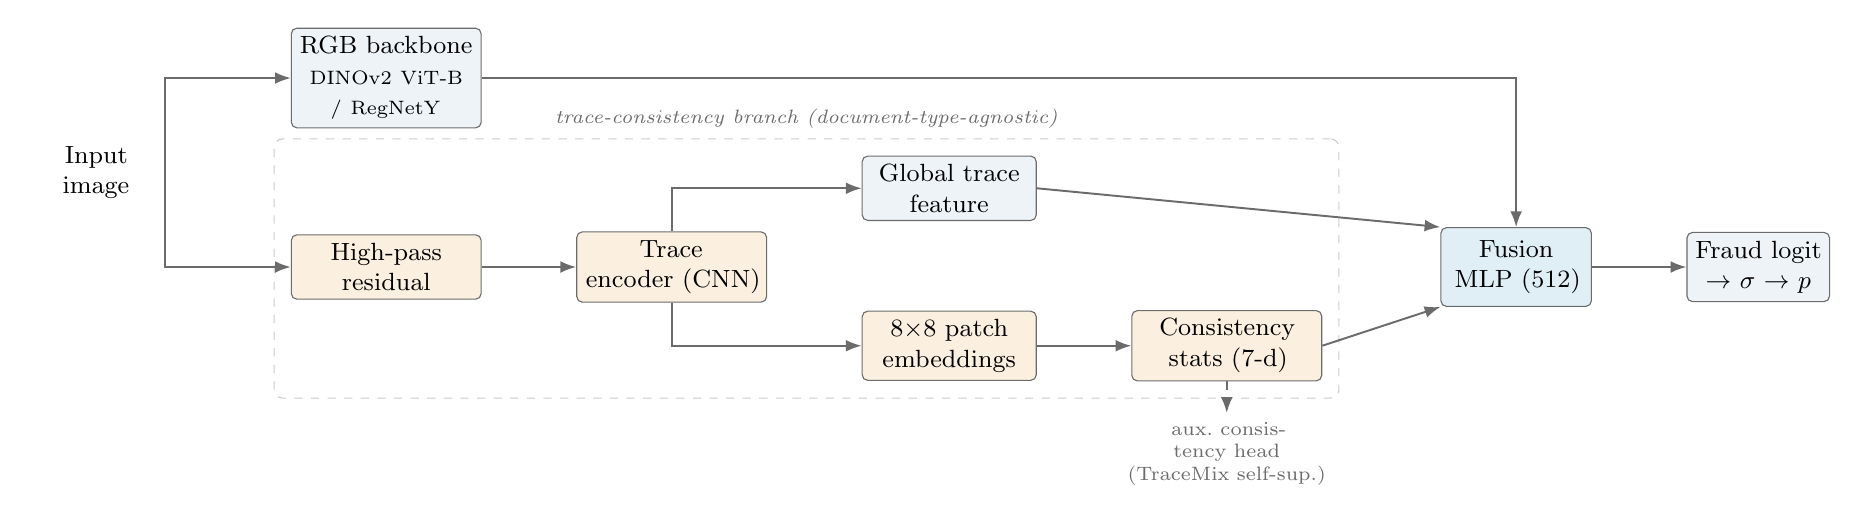
\begin{tikzpicture}[
  font=\small,
  block/.style={draw=axgray, rounded corners=2pt, fill=blockbg, align=center,
                minimum height=8mm, inner sep=3pt, text width=22mm},
  trace/.style={draw=axgray, rounded corners=2pt, fill=tracebg, align=center,
                minimum height=8mm, inner sep=3pt, text width=22mm},
  fuse/.style={draw=axgray, rounded corners=2pt, fill=cpub!12, align=center,
               minimum height=10mm, inner sep=3pt, text width=17mm},
  io/.style={align=center, text width=15mm},
  arr/.style={-{Latex[length=2mm]}, axgray, line width=0.7pt},
  node distance=7mm and 12mm,
]
\node[io] (img) {Input\\image};
\node[block, right=16mm of img, yshift=12mm] (rgb) {RGB backbone\\{\scriptsize DINOv2 ViT-B / RegNetY}};
\node[trace, right=16mm of img, yshift=-12mm] (hp) {High-pass\\residual};
\node[trace, right=of hp] (te) {Trace\\encoder (CNN)};
\node[block, right=of te, yshift=10mm, text width=20mm] (gt) {Global trace\\feature};
\node[trace, right=of te, yshift=-10mm, text width=20mm] (patch) {$8{\times}8$ patch\\embeddings};
\node[trace, right=of patch, text width=22mm] (cons) {Consistency\\stats (7-d)};
\node[fuse, right=15mm of cons, yshift=10mm] (fusion) {Fusion\\MLP (512)};
\node[block, right=12mm of fusion, text width=16mm] (out) {Fraud logit\\$\rightarrow\sigma\rightarrow p$};
\node[align=center, below=4mm of cons, text width=26mm, font=\scriptsize, text=axgray]
  (aux) {aux.\ consistency head\\(TraceMix self-sup.)};

\draw[arr] (img.east) |- (rgb.west);
\draw[arr] (img.east) |- (hp.west);
\draw[arr] (hp) -- (te);
\draw[arr] (te) |- (gt.west);
\draw[arr] (te) |- (patch.west);
\draw[arr] (patch) -- (cons);
\draw[arr] (rgb.east) -| (fusion.north);
\draw[arr] (gt.east) -- (fusion.north west);
\draw[arr] (cons.east) -- (fusion.south west);
\draw[arr] (fusion) -- (out);
\draw[arr, dashed] (cons.south) -- (aux.north);

\begin{scope}[on background layer]
  \node[draw=axgray!35, dashed, rounded corners=3pt, fit=(hp)(te)(gt)(patch)(cons),
        inner sep=6pt,
        label={[font=\scriptsize\itshape, text=axgray]above:trace-consistency branch (document-type-agnostic)}] {};
\end{scope}
\end{tikzpicture}}
\caption{The Double-Trace Consistency detector (DTC). A pretrained RGB backbone is fused with a high-pass
forensic branch. The patch-consistency statistics measure whether the acquisition trace is internally
coherent. This
signal does not depend on document-type appearance. Each deployed model is one such detector. The
private-best model averages three of them (Section~\ref{sec:diversity}).}
\label{fig:arch}
\end{figure*}

\subsection{Double-Trace Consistency detector}
\label{sec:dtc}
Each detector (Fig.~\ref{fig:arch}) combines an ImageNet/DINOv2-pretrained RGB backbone with a forensic
branch. The forensic branch applies a Gaussian high-pass residual and a small strided CNN
(\texttt{TraceEncoder}) that keeps the spatial layout. It produces (i) a global trace feature and (ii) an
$8\times8$ grid of L2-normalised patch trace embeddings $\{z_i\}$. We take the off-diagonal pairwise cosine
similarities of $\{z_i\}$ and compute a 7-dimensional \textbf{consistency statistic} $s(x)$ (mean, standard
deviation, minimum, low percentiles, and per-patch max-similarity summaries). The name comes from the two
uses of the high-pass trace: the global trace feature and the patch-level consistency signal $s(x)$. A
genuine capture, including
a legitimately re-captured one, has a uniform trace. A locally edited and reprinted forgery does not. The
statistic $s(x)$ does not depend on the document type, so an unseen-type genuine document is not flagged
only because it looks unfamiliar. The fraud logit fuses
$[\,\text{RGB feature}\,;\,\text{global trace}\,;\,s(x)\,]$ through an MLP
($\text{Linear}\!\rightarrow\!512\!\rightarrow\!\text{GELU}\!\rightarrow\!\text{Dropout}(0.1)\!\rightarrow\!\text{Linear}\!\rightarrow\!1$).
An auxiliary head on $s(x)$ is trained on self-supervised \texttt{TraceMix} coherent/incoherent labels,
which are independent of the fraud label. The branch does not depend on the backbone, so any RGB family can
host it.

\subsection{Capture robustness by data, not architecture}
\label{sec:capture}
Robustness to captured documents comes from \emph{data and augmentation}, not from architecture or loss
changes (Section~\ref{sec:rejected}). The private-best models train on FREUID plus diverse real
captured-genuine corpora (Section~\ref{sec:data}) with heavy print-and-capture augmentation and FDA domain
randomisation~\cite{fda}. With probability $0.4$ we swap the low-frequency amplitude spectrum of an image
with a donor of a \emph{different} document type ($\beta\in[0.01,0.08]$). This randomises the type
appearance and keeps the forensic phase.

\subsection{Diversity-axis ensembling}
\label{sec:diversity}
A single capture detector is limited. The gain comes from averaging backbones that are \emph{decorrelated
along independent axes}. We treat architecture family and input resolution as two separate diversity axes.
Two ViT-B detectors at different resolutions are strongly correlated (Spearman $\rho\!\approx\!0.79$). A
pure-CNN family at a different resolution is much less correlated ($\rho\!\approx\!0.5$--$0.7$). Adding such
a member crosses both axes at once, and it gives the largest ensemble gain (Fig.~\ref{fig:ladder}). Extra
\emph{seeds} of the same architecture and resolution ($\rho\!>\!0.99$) do not help. This principle applies
to both tracks (Section~\ref{sec:results}).

\subsection{The submitted model}
\label{sec:models}
We submit one model, the \textbf{private-best} ensemble: a probability average of three DTC detectors,
selected on a captured proxy: ViT-B/14 DINOv2 at $896$ and $1120$\,px, and RegNetY-160 at $1120$\,px. The
two ViT-B anchors stabilise the operating point, because their score is stable across seeds. The
decorrelated RegNetY adds the ranking gain. Across three seeds, this configuration had the smallest
variance among the candidates. This is the model shipped in the reproducibility container.

For analysis we also build a \textbf{public-best} ensemble that we do \emph{not} submit: a diversity-axis
ensemble (ViT-L, ConvNeXt~V2, ViT-Giant across resolutions) with a \emph{field-tamper} augmentation that
targets born-digital tampering. It tops the public leaderboard but collapses on captured data
(Section~\ref{sec:antagonism}), so it is a reference, not our submission.

\subsection{Score calibration}
\label{sec:calib}
Each detector outputs a fraud logit. A sigmoid maps it to a per-model probability. The submission score is
the arithmetic mean of the ensemble probabilities. We apply no temperature or learned calibration, and no
post-processing differs between train and test time. Unreadable images are assigned $0.5$, so every input
gives exactly one finite score in $[0,1]$.

\section{Data}
\label{sec:data}
We use the official FREUID \texttt{train/} images and \texttt{train.csv} metadata (Kaggle competition
\texttt{the-freuid-challenge-2026-ijcai-ecai}). The private-best models also train on diverse
\emph{captured-genuine} corpora (moderate upweight, no external fraud labels): MIDV-500~\cite{midv500},
MIDV-2019, MIDV-Holo, MIDV-2020, and BID (Brazilian CNH/RG/CPF photographs). We combine these with FREUID
into a single manifest. FantasyID, a public research dataset of fantasy ID cards (Idiap), is held out as a leakage-free
\emph{captured proxy}. It is a separate corpus, so we never train on it; we use it only for model selection.
Its composition is described in the Validation paragraph below. All corpora are used under their public
research licenses, and the pretrained weights under their upstream licenses.

\paragraph{Validation.} The public leaderboard reflects the born-digital distribution, so it does not
predict the captured private set (Section~\ref{sec:antagonism}). We therefore select the private-best model
on a captured proxy, the FantasyID test split: 1{,}295 images across six document styles (465 genuine cards
that are physically printed and photographed, and 830 GenAI-manipulated versions with face-swap or text
edits). We chose FantasyID because it matches the two stated properties of the private test
(Section~\ref{sec:intro}): its genuine cards are captured rather than born-digital, and its document styles
differ from the five FREUID training types. We do not claim that FantasyID and the private set share the
same distribution, and FantasyID is not an organizer-recommended proxy; its attack types in particular may
differ from the private test. We therefore use it only for model selection and read its FREUID score as an
indicative lower bound. We hold out a random $10\%$ split of the training manifest only for logging. The
private set is not available at submission time, so proxy selection is the only option.

\section{Inference}
\label{sec:inference}
The container entrypoint indexes a flat directory of images. It runs the three checkpoints (build with
\texttt{pretrained=False}, load embedded weights, forward pass, sigmoid) and writes the per-image
probability average as \texttt{id,label}. Test-time preprocessing is a plain resize to the native
resolution with ImageNet normalisation. The deployed models use no tiling, no multi-crop, and no test-time
augmentation. The device is CUDA if available, else CPU. The per-model batch size follows the training
config. Unreadable images are assigned $0.5$. The exact command is in Section~\ref{sec:repro}.

\section{Results}
\label{sec:results}

\subsection{Main results}
Table~\ref{tab:results} reports the submitted private-best model and the public-best reference on both
splits. The private-best model reduces a two-backbone baseline by about half on the captured proxy, and it
stays well above chance on born-digital data. The public-best reference reaches a public FREUID Score of
$0.00041$ (with three models; $0.00039$ for the full ensemble), but it collapses on captured data, so we do
not submit it.

\begin{table}[t]
\centering
\small
\setlength{\tabcolsep}{6pt}
\caption{Main results. FREUID Score $\downarrow$ (lower is better). We submit the private-best model; the
public-best is a public-leaderboard reference we do not submit, because it collapses on captured data
(Fig.~\ref{fig:antagonism}). Captured-proxy figures are a small cross-corpus lower bound.}
\label{tab:results}
\begin{tabular}{lcc}
\toprule
Model & Public LB $\downarrow$ & Captured proxy $\downarrow$ \\
\midrule
Private-best (submitted)               & $0.169$          & \textbf{${\approx}0.22$--$0.27$} \\
Public-best (reference, not submitted) & \textbf{0.00041} & ${\approx}0.99$\,{\footnotesize(chance)} \\
\bottomrule
\end{tabular}
\end{table}

\subsection{Each model works on only one distribution}
\label{sec:antagonism}
Fig.~\ref{fig:antagonism} plots each model on both distributions. The two lines cross. The public-best
model is strong on born-digital data ($0.00041$) but at chance on captured data (about $0.99$; a random
classifier scores about $0.99$ on APCER@1\%BPCER). The reason is that the public-best model relies on
born-digital forensic cues, such as fine editing traces and JPEG discontinuities. Print-and-capture
re-acquisition overwrites these cues with a uniform capture signature, so they no longer separate genuine
from fraud. The private-best model shows the opposite order. The gap between the two models is about
$400\times$ on the public set, and the order fully reverses on the captured proxy. A single model therefore
cannot serve both distributions, and the public score does not predict private performance. The
private-best model stays well above chance on born-digital data ($0.169$), so it is our submitted model: it
does not collapse on either split, and it is the stronger choice on the captured and unseen-type content
that the private split contains and the public split does not.

\begin{figure}[t]
\centering
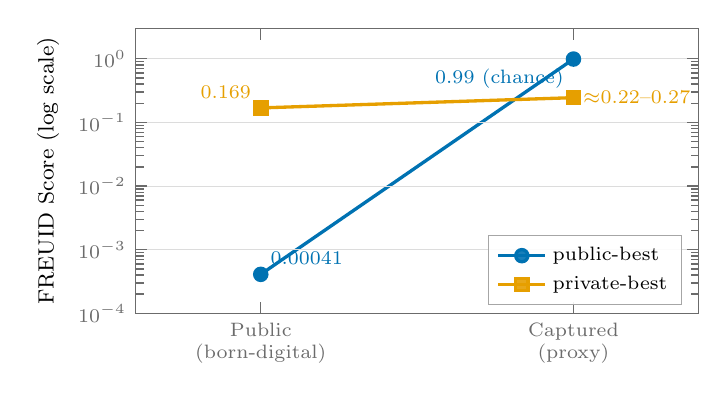
\begin{tikzpicture}
\begin{axis}[paperaxis, ymode=log,
  xmin=-0.4, xmax=1.4, xtick={0,1},
  xticklabels={Public\\(born-digital), Captured\\(proxy)},
  xticklabel style={align=center},
  ymin=1e-4, ymax=3, ylabel={FREUID Score (log scale)},
  ytick={1e-4,1e-3,1e-2,1e-1,1},
  legend pos=south east,
]
\addplot[cpub, line width=1.2pt, mark=*, mark size=2.2pt] coordinates {(0,0.00041) (1,0.99)};
\addplot[cpriv, line width=1.2pt, mark=square*, mark size=2.2pt] coordinates {(0,0.169) (1,0.245)};
\node[cpub,  font=\scriptsize, anchor=south west] at (axis cs:0,0.00041) {0.00041};
\node[cpub,  font=\scriptsize, anchor=north east] at (axis cs:1,0.99) {0.99 (chance)};
\node[cpriv, font=\scriptsize, anchor=south east] at (axis cs:0,0.169) {0.169};
\node[cpriv, font=\scriptsize, anchor=west] at (axis cs:1,0.245) {$\approx$0.22--0.27};
\legend{public-best, private-best}
\end{axis}
\end{tikzpicture}
\caption{Each model fits only one distribution. A model is strong (low) on its own distribution and weak
(high) on the other, so the two lines cross. Lower is better.}
\label{fig:antagonism}
\end{figure}

\subsection{Diversity axes beat seeds (measured on the public leaderboard)}
\label{sec:public-abl}
The diversity-axis principle is easiest to measure on the public leaderboard, where the labels are real.
Fig.~\ref{fig:progression} traces the public FREUID Score as we add each component to the public-best
reference. The field-tamper augmentation gives the first large drop. Adding architecture diversity, then
resolution diversity, and then an axis-crossing member each lowers the score further. Seed replicas (not
shown) do not change the score. We apply the same principle to the submitted model
(Section~\ref{sec:private-abl}).

\begin{figure}[t]
\centering
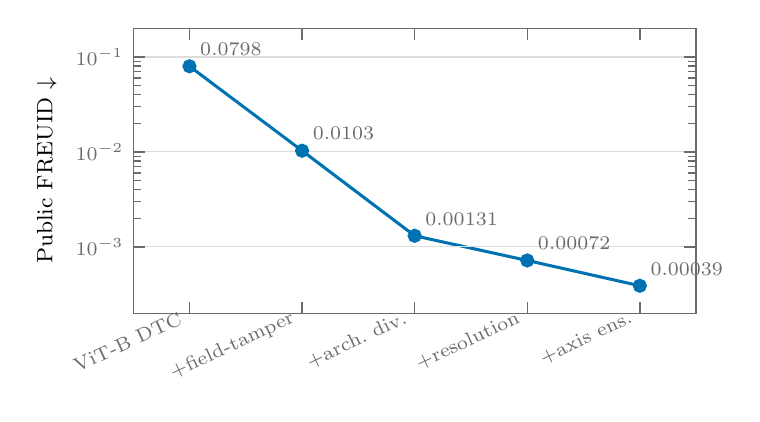
\begin{tikzpicture}
\begin{axis}[paperaxis, ymode=log,
  xmin=0.5, xmax=5.5, xtick={1,2,3,4,5},
  xticklabels={ViT-B DTC, +field-tamper, +arch.\ div., +resolution, +axis ens.},
  xticklabel style={rotate=25, anchor=east, font=\scriptsize},
  ymin=2e-4, ymax=0.2, ylabel={Public FREUID $\downarrow$},
  ytick={1e-3,1e-2,1e-1},
]
\addplot[cpub, line width=1.1pt, mark=*, mark size=2pt,
  point meta=explicit symbolic, nodes near coords,
  every node near coord/.append style={font=\scriptsize, color=axgray, anchor=south west}]
  coordinates {(1,0.0798)[0.0798] (2,0.0103)[0.0103] (3,0.00131)[0.00131]
               (4,0.00072)[0.00072] (5,0.00039)[0.00039]};
\end{axis}
\end{tikzpicture}
\caption{The diversity-axis principle on the public-best reference. Each added component lowers the public
FREUID Score. The full ensemble reaches $0.00039$; the three-model version scores $0.00041$. This model is
not submitted.}
\label{fig:progression}
\end{figure}

\subsection{Ensemble ladder (submitted model)}
\label{sec:private-abl}
Fig.~\ref{fig:ladder} shows the same principle on the submitted model, measured on the captured proxy. We
start from two correlated ViT-B detectors. Each new decorrelated family lowers the proxy FREUID Score. The
axis-crossing member (RegNetY-160 at $1120$\,px, a new family and a new resolution) gives the final step and
reduces the two-ViT baseline by about half.

\begin{figure}[t]
\centering
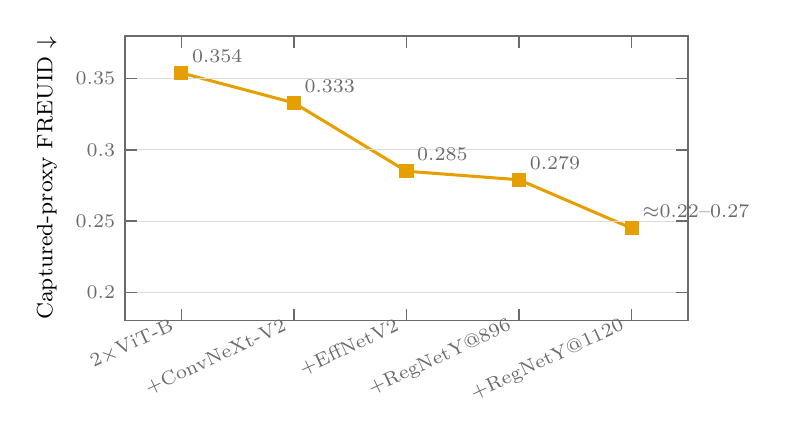
\begin{tikzpicture}
\begin{axis}[paperaxis,
  xmin=0.5, xmax=5.5, xtick={1,2,3,4,5},
  xticklabels={$2{\times}$ViT-B, +ConvNeXt-V2, +EffNetV2, +RegNetY@896, +RegNetY@1120},
  xticklabel style={rotate=25, anchor=east, font=\scriptsize},
  ymin=0.18, ymax=0.38, ylabel={Captured-proxy FREUID $\downarrow$},
]
\addplot[cpriv, line width=1.1pt, mark=square*, mark size=2pt,
  point meta=explicit symbolic, nodes near coords,
  every node near coord/.append style={font=\scriptsize, color=axgray, anchor=south west}]
  coordinates {(1,0.354)[0.354] (2,0.333)[0.333] (3,0.285)[0.285]
               (4,0.279)[0.279] (5,0.245)[$\approx$0.22--0.27]};
\end{axis}
\end{tikzpicture}
\caption{Ensemble ladder for the submitted model. Adding decorrelated architecture/resolution members lowers
the captured-proxy FREUID Score. The last point is a range. The plotted value is its midpoint.}
\label{fig:ladder}
\end{figure}

\subsection{Approaches evaluated and rejected}
\label{sec:rejected}
We also tested approaches that did not help, and we dropped them. Submitting the public-best ensemble on
captured data was capture-blind (about chance). Adding MIDV-2020 to the capture mix gave no gain, because
of a distribution mismatch. A learned domain router keyed on framing and context, and it misrouted cropped
captured images. Warm-starting the capture model from the public-best checkpoint gave a worse peak, because
the fraud-specific features do not survive re-capture. Architecture and loss levers on the capture axis
(focal loss~\cite{focal}, CDC convolutions~\cite{cdcn}, MixStyle~\cite{mixstyle}) did worse than the
data-diversity recipe.

\section{Reproducibility}
\label{sec:repro}
The reproducibility container ships the private-best model. The weights are baked into the image, and the
models build with \texttt{pretrained=False}. The container therefore runs with \texttt{--network none} (no
runtime downloads) and writes only to \texttt{/submissions}.
\begin{itemize}[leftmargin=1.2em,itemsep=1pt,topsep=2pt]
  \item \textbf{Environment (pinned):} \texttt{torch==2.12.0} (CUDA 13), \texttt{timm==1.0.27},
        \texttt{albumentations==2.0.8}, \texttt{opencv-python-headless==4.13.0}, \texttt{numpy==2.4.6},
        \texttt{pandas==3.0.3}, \texttt{scipy==1.17.1}, \texttt{scikit-learn==1.9.0},
        \texttt{pillow==12.2.0}, \texttt{pyyaml==6.0.2}, \texttt{pyarrow}; Python $\geq 3.11$.
  \item \textbf{Hardware / runtime:} training on $2\times$ NVIDIA RTX PRO 6000 (Blackwell, 96\,GB);
        inference uses a single GPU. The CPU fallback works but is slow.
  \item \textbf{Randomness:} global seed $42$. CUDA/cuDNN and AMP add minor non-determinism, within the
        proxy's seed noise.
  \item \textbf{Repository:} \url{https://github.com/hoppery/freuid-challenge-2026} (MIT license; the frozen
        commit SHA is in our reproducibility reply).
\end{itemize}

\noindent\textbf{Build and run (organizer contract):}
{\footnotesize
\begin{verbatim}
docker build -t freuid-repro:local .
docker run --network none \
  -v <flat_images>:/data:ro \
  -v "$(pwd)/out":/submissions \
  freuid-repro:local        # -> out/submission.csv  (id,label)
\end{verbatim}}

\section{Team and contributions}
\label{sec:team}
Both authors contributed to the method, the experiments, and the manuscript. Su-Yong An (corresponding
author) led model development, training, and evaluation. Lae-Kyoung Lee contributed to the methodology, the
analysis, and the manuscript.

\section*{Acknowledgments}
This work was supported by Electronics and Telecommunications Research Institute (ETRI) grant funded by the
Korean government [26ZD1160, Advancement and Commercialization of Daegu-Gyeongbuk Regional Strategic
Industries (Robots, Mobility, AI, Medical, etc.)].

\bibliographystyle{plain}
\bibliography{references}

\appendix
\section{Hyperparameters}
\label{app:hparams}
\begin{table}[H]
\centering
\small
\setlength{\tabcolsep}{5pt}
\caption{Per-model hyperparameters of the private-best ensemble. Shared: AdamW, weight decay $0.05$, cosine
LR schedule, 3 epochs, seed 42, AMP, DTC consistency weight $\lambda_{\text{dtc}}{=}0.5$,
\texttt{tracemix\_p}{=}0.5, \texttt{fda\_p}{=}0.4, heavy print-and-capture augmentation.}
\label{tab:hparams}
\begin{tabular}{lccc}
\toprule
Hyperparameter & ViT-B @896 & ViT-B @1120 & RegNetY-160 @1120 \\
\midrule
Backbone      & \multicolumn{2}{c}{\texttt{vit\_base\_patch14\_reg4\_dinov2}} & \texttt{regnety\_160.tv2\_in1k} \\
Image size    & 896 & 1120 & 1120 \\
Batch size    & 24  & 12   & 8 \\
Learning rate & $1{\times}10^{-4}$ & $1{\times}10^{-4}$ & $5{\times}10^{-5}$ \\
Weight decay  & 0.05 & 0.05 & 0.05 \\
Epoch used    & 2 & 2 & 1 \\
Backbone freezing & last 2 blocks $+$ norm & last 2 blocks $+$ norm & full fine-tune \\
Seed          & 42 & 42 & 42 \\
\bottomrule
\end{tabular}
\end{table}

\section{Additional ablations}
\label{app:ablations}
See Figs.~\ref{fig:progression} and~\ref{fig:ladder} (diversity-axis contributions on each track) and the
rejected-approaches list in Section~\ref{sec:rejected}. Further ablations (capture-source diversity and
resolution sweeps) are available in the repository notes.

\end{document}
